% Copyright (C) 2014 by Thomas Auzinger <thomas.auzinger@cg.tuwien.ac.at>

\documentclass[draft,final]{vutinfth} % Remove option 'final' to obtain debug information.

% Extended LaTeX functionality is enables by including packages with \usepackage{...}.
\usepackage{fixltx2e}  % Provides fixes for several errors in LaTeX2e.
\usepackage{amsmath}   % Extended typesetting of mathematical expression.
\usepackage{amssymb}   % Provides a multitude of mathematical symbols.
\usepackage{mathtools} % Further extensions of mathematical typesetting.
\usepackage{microtype} % Small-scale typographic enhancements.
\usepackage{enumitem}  % User control over the layout of lists (itemize, enumerate, description).
\usepackage{multirow}  % Allows table elements to span several rows.
\usepackage{booktabs}  % Improves the typesettings of tables.
\usepackage[ruled,linesnumbered,algochapter]{algorithm2e} % Enables the writing of pseudo code.
\usepackage{nag}       % Issues warnings when best practices in writing LaTeX documents are violated.
\usepackage{hyperref}  % Enables cross linking in the electronic document version. This package has to be included second to last.
\usepackage[acronym,toc]{glossaries} % Enables the generation of glossaries and lists fo acronyms. This package has to be included last.

\usepackage{tikz}
\usepackage{placeins}
\usepackage{amsmath}

\newcommand{\hl}{\par\vspace{6pt}} %used within the same context, as new paragraph
\newcommand{\cl}{\par\vspace{12pt}} %used between paragraphs with the same topic, but not textually flowing into each other
\newcommand{\dl}{\par\vspace{24pt}} %used to get to the next topic
\setlength{\parindent}{0pt} %should remove all intendations

\setsecnumdepth{subsection} % enumerate subsections

% Use an optional index
\makeindex
% Use an optional glossary
\makeglossaries
%\glstocfalse % remove the glossaries from the table of contents

% Set persons with 4 arguments:
%  {title before name}{name}{title after name}{gender}
%  where both titles are optional (i.e. can be given as empty brackets {})
\setauthor{}{Patrick Bellositz}{}{male}
\setadvisor{Ao.Prof.Dipl.-Ing.Dr.techn.}{Christian Georg Ferm{\"u}ller}{}{male}

% Required data
\setaddress{Eichkogelstra{\ss}e 10/10/9, 2353 Guntramsdorf}
\setregnumber{1027108}
\setdate{01}{06}{2015}
\settitle{Abstract Argumentation Frameworks}{Abstract Argumentation Frameworks} % sets English and German version of the title (both can be English or German)

\setthesis{bachelor}

% For bachelor and master
\setcurriculum{Software \& Information Engineering}{Software \& Information Engineering} % sets the English and German name of the curriculum

\begin{document}

\frontmatter % switches to roman numbering
% The structure of the thesis has to conform to
%  http://www.informatik.tuwien.ac.at/dekanat

%\addtitlepage{naustrian}
\addtitlepage{english} % English title page
\addstatementpage

\begin{acknowledgements*}
I want to thank my family for supporting me and Dr. Ferm{\"u}ller for guiding me in the process of creating this thesis.
\end{acknowledgements*}

\begin{abstract*}
This bachelor thesis explains the concept of the abstract argumentation framework, its properties as well as its extensions. It further analyzes the relations between different types of extensions.\hl
The main part of the thesis is the modelling of the explained concepts as code and the developement of a JAVA application which is capable of creating custom argumentation frameworks, their visualisation as graphs and the computation of extensions. The application is created in a way such that students can study argumentation frameworks in an easily digestable way including step-by-step explanations of how the extensions are computed accompanied by colored highlighting of important aspects of the frameworks' graphs.\\ %TODO work in progress
\end{abstract*}

% Select the language of the thesis, e.g., english or naustrian.
\selectlanguage{english}

% Add a table of contents (toc)
\tableofcontents* % starred version, i.e., \tableofcontents*, removes the self-entry

% Switch to arabic numbering and start the enumeration of chapters in the table of content.
\mainmatter

\chapter{Introduction}
Most humans argue on a daily basis. Often argument is followed by counter-argument is followed by another counter-argument until one of the participants is defeated.\hl
Each of these arguments consists of the following ingredients:

\begin{itemize}
	\item Premises
	\item Conclusions
\end{itemize}

A counter-argument now tries to either disprove a premise or a conclusion. For example:\hl
\[
	\underbrace{\text{All birds can fly.}}_\text{premise}\text{ }
	\underbrace{\text{Tweety is a bird.}}_\text{premise}\text{ }
	\underbrace{\text{Therefore Tweety can fly.}}_\text{conclusion}
\]
One now could bring up the fact, that penguins are birds that can't fly, thus disproving the first premise. It could also be argued, that Tweety is not a bird, but rather a virtual character which can not be compared to the real world, attacking the second premise.\hl

Now lets change our argument slightly:\hl
\[
	\underbrace{\text{All birds can fly.}}_\text{premise}\text{ }
	\underbrace{\text{Tweety can fly.}}_\text{premise}\text{ }
	\underbrace{\text{Therefore Tweety is a bird.}}_\text{conclusion}
\]\hl
Now the conclusion of the argument could also be attacked.\cl

In reality arguments are not always contructed in a way, where premises and conclusions can so easily be spotted, because they are often implicit. For example\hl
\[\text{Dirty things need to be cleaned. The floor is dirty.}\]\hl
consists only of premises and does not have an explicit conclusion.\hl
While humans automatically grasp implicit premises or conclusions for simple arguments, this is not always the case. Complicated discussions or negotiations often are too complex to immediately understand. Computers gernerally also don't understand arguments very well. To use the optimal set of arguments one could now formalise the arguments and especially how they relate to each other to come to an optimal solution.\hl %did I connect dung well enough with complex argumentation structures?
In this paper we look at the concept of argumentation frameworks as proposed by Dung in {year}. %reference and year here
Following that we look at an application written for this thesis and specifically designed to illustrate and explain how such sets of arguments can be obtained.

\chapter{Definitions}

To work with argumentation frameworks, first we must define their properties. This section will lay out the basic structure of argumentation frameworks as well as provide extension types for further analysis.\dl

\textbf{Definition 1.} An \emph{argumentation framework} $F$ is a pair $(A,R)$, where $A$ is a set of arguments and $R$ is a set of attack relations.\cl

\textbf{Definition 2.} \emph{Attack relations} $R\subseteq A\times A$ represent attacks. The pair $(a,b)$, where $a,b\in A$ means $a$ \emph{attacks} $b$.\cl

\textbf{Remark 1.} Let $S$ be a set of arguments. If $a\in S$ and there is an attack $(a,b)\in R$ we say $S$ \emph{attacks} $b$.\cl

\textbf{Example 1.} Imagine we have 3 arguments $a_1$, $a_2$, and $b$.\hl
			\begin{tabular}{p{0.5cm}p{0.5cm}l}
			& $a_1$ & = ''Blue is the most beautiful of all colors.''\\
			& $b$ & = ''No, black is much more beautiful!''\\
			& $a_2$ & = ''That's wrong, black isn't even a color.''
			\end{tabular}\hl
These arguments obvioucly contain 2 attacks. Argument $b$ attacks argument $a_1$ and in turn argument $a_2$ attacks argument $b$.\hl
This results in the framework $F=(A,R)$, where $A=\{a_1,a_2,b\}$ and $R=\{(b,a_1),(a_2,b)\}$.\cl

A big argument framework in might become hard to read with increasing set sizes, so it is also possible to represent every framework as a graph $(V,E)$, where $V=A$ and $E=R$. The graph of our example looks like this:

\FloatBarrier
	\begin{figure}[!htb]
		\centering
		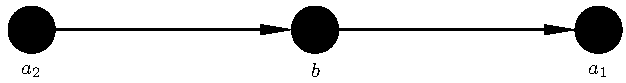
\includegraphics[width=\linewidth]{graphs/ex1.pdf}
		\caption{An argument framework about colors.}
	\end{figure}
\FloatBarrier

Depending on their properties, arguments can be grouped into \emph{extensions} in order to obtain additional knowledge about the framework.\dl

As a basis we introduce the \emph{conflict-free set}, since no extension should contain arguments that are in conflict with each other (i.e. there can't be attacks within an extension).\cl

\textbf{Definition 3.} Let $S$ be a set of arguments. It is \emph{conflict-free}, if $\forall a \forall b\ a,b\in S, (a,b)\notin R$.\\
The set of all conflict-free sets of an argumentation framework $F$ is denoted $cf(F)$.\cl

\textbf{Example 2.} (Continuation of Example 1) As no argument attacks itself, $\{a_1\}$, $\{a_2\}$ and $\{b\}$ each are conflict-free. $\{a_1,a_2\}$ is also a conflict-free set, since there exists no attack relation containing $a_1$ and $a_2$. The empty set is always conflict-free.\hl
Since there is an attack relation between $b$ and each of the other arguments, there are no other conflict-free sets.\hl
It follows that $cf(F)=\{\emptyset,\{a_1\},\{a_2\},\{b\},\{a_1,a_2\}\}$.\dl

To be able to find a set of arguments that can't be reasoned against, it does not suffice if that set is only not in itself conflicted, but each argument should also not be an invitation for an easy counter-argument. Therefore it is necessary to only accept arguments into a set that don't hurt its defendability.\cl

\textbf{Definition 4.} An argument $a$ is \emph{defended} by a set $S$, if for every attack $(b,a)\in R$ there is an attack $(c,b)$, where $c\in S$. If this is the case $S$ \emph{defends} $a$.\dl

\textbf{Definition 5.} Let $S$ be a conflict-free set. It is called an \emph{admissible extension} if it defends each $a\in S$.\\
The set of all admissible extensions of an argumentation framework $F$ is denoted $adm(F)$.\dl

\textbf{Example 3.} (Continuation of Example 2) Of the conflict-free sets only $\{a_2\}$ and \(\emptyset\) don't get attacked. They are admissible. $\{a_1,a_2\}$ gets attacked via the attack relation $(b,a_1)$, but $a_1$ gets defended through $(a_2,b)$, making it also admissible.\\
$\{b\}$ and $\{a_1\}$ are not admissible since they don't defend their arguments.\hl
It follows that $adm(F)=\{\emptyset,\{a_1,a_2\},\{a_2\}\}$.\dl

Using admissible extensions we now can reduce the number of relevant extensions by eliminating redundant extensions, all containing the same arguments, by only taking the biggest ones, that include smaller extensions. The resulting preferred extensions are an example of a credulous reasoning, since they contain all arguments that are contained in admissible extensions.\cl

\textbf{Definition 6.} Let $S$ be an admissible extension. It is called a \emph{preferred extension} if for each $S'\subseteq A$, that is an admissible extension, $S\not\subset S'$.\\
The set of all preferred extensions of an argumentation framework $F$ is denoted $pr(F)$.\cl

\textbf{Example 4.} (Continuation of Example 3) Since $\emptyset\subset\{a_2\}$, \(\emptyset\) is not a preferred extension. $\{a_2\}\subset\{a_1,a_2\}$, therefore $\{a_2\}$ is not a preferred extension. Since all other admissible extensions are proper subsets of $\{a_1,a_2\}$, it is a preferred extension.\hl
It follows that $prf(F)=\{\{a_1,a_2\}\}$.\hl
As we can see, all arguments contained in admissible extensions still are contained in a preferred extension, even though the number of results is smaller.\dl

Additionally we can define a stricter version of the admissible extension, that not only requires arguments to be defended, but also needs to attack all arguments not contained within it.\cl

\textbf{Definition 7.} Let $S$ be a conflict-free set. It is called a \emph{stable extension} if for each $a\not\in S$ there is exists an attack $(b,a)\in R$ where $b\in S$.\\
The set of all stable extensions of an argumentation framework $F$ is denoted $st(F)$.\cl

\textbf{Example 5.} (Continuation of Example 2) The conflict-free sets $\emptyset$ and $\{a_1\}$ don't attack any of the other arguments, $\{a_2\}$ only attacks $\{b\}$, missing an attack on $\{a_1\}$. $\{b\}$ misses an attack on $\{a_2\}$. They are not stable extensions.\\
$\{a_1,a_2\}$ attacks all other arguments in $\{b\}$ (attack relation $(a_2,b)$) and therefore is a stable extension.\hl
It follows that $st(F)=\{\{a_1,a_2\}\}$.\dl

In contrast to credulous reasoning stands sceptical reasoning. The extension fitting sceptical reasoning within the context of argument frameworks is the complete extension.\cl

\textbf{Definition 8.} Let $S$ be an admissible extension. It is called a \emph{complete extension} if for each $a\not\in S$, $S\cup \{a\}$ is not an admissible extension.\\
The set of all complete extensions of an argumentation framework $F$ is denoted $co(F)$.\cl

\textbf{Example 6.} (Continuation of Example 3) The admissible extension $\emptyset$ is not a complete extension because it defends $a_2$ which it doesn't contain. $\{a_2\}$ defends $a_1$ and is therefore also not a complete extension.\\
$\{a_1,a_2\}$ attacks $b$ and as there are no other arguments which could be defended it is a complete extension.\hl
It follows that $co(F)=\{\{a_1,a_2\}\}$.\dl

As before, we can again reduce the number of relevant extensions. In this case we search for the common denominator, meaning exactly those arguments all complete extensions can ``agree'' on. This results in the grounded extension\cl

\textbf{Definition 9.} The (unique) \emph{grounded extension} is defined by $\bigcap\limits_{i=1}^n{S_i}$, where $\{S_1,...,S_n\}$ is the set of all complete extensions.\\
The grounded extension of an argumentation framework $F$ is denoted $gr(F)$\cl

\textbf{Example 7.} (Continuation of Example 6) Since there is only one complete extension $\{a_1,a_2\}$, it also is the grounded extension $gr(F)$.\dl

\chapter{Observations}

As we have seen in the previous section, often there may be overlaps between the different extension types. In this section we will discuss those relations between extension types. Additionally we will explore their unique features.\dl

As per the definitions of the extension there are the following relations:
\begin{align} %find structure that instead centers
	adm(F)\subseteq cf(F)\\
	st(F)\subseteq cf(F)\\
	prf(F)\subseteq adm(F)\\
	co(F)\subseteq adm(F)
\end{align}\dl

\textbf{Lemma 1.} %TODO provide proof
Each stable extension is a preferred extension, but not every preferred extension is a stable extension.\\
\begin{align}
	st(F)\subseteq prf(F)\\
	prf(F)\not\subseteq st(F)
\end{align}
Therefore each stable extension also is an admissible extension.\cl

\textbf{Example 7.} Let $F$ be an argumentation framework $(A,R)$ such that $A={a,b,c}$ and $R={(b,a),(b,c),(a,a),(c,b)}$.

\FloatBarrier
	\begin{figure}[!htb]
		\centering
		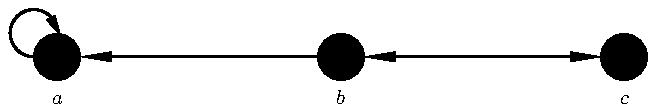
\includegraphics[width=\linewidth]{graphs/ex2.pdf}
		\caption{Example for the difference between stable and preferred extensions}
	\end{figure}
\FloatBarrier

It can be computed that $cf(F)=adm(F)=\{\{b\},\{c\}\}$. So we only have to consider two extensions for further computations.\hl
As can be seen, $\{b\}$ is the only conflict-free set that attacks all other arguments. Therefore $st(F)=\{\{b\}\}$.\hl
We know that $\{b\}$ has to be a preferred extension, because of Lemma 1. $\{c\}$ attacks only it's attacker $b$, but not $a$. Therefore it is preferred and $prf(F)=\{\{b\},\{c\}\}$.\dl

\textbf{Lemma 2.} %check for something better, needs proof?
The grounded extension is always admissible. %and, something?
\begin{align}
	gr(F)\subseteq adm(F)
\end{align}

%others, TODO split within text

\begin{align}
	co(F)\not\subseteq prf(F)\\
	prf(F)\not\subseteq co(F)\\
	\exists F\ prf(F)\cap co(F) \not = \emptyset\\
	\exists F\ st(F)\cap co(F) \not = \emptyset 
\end{align}

\FloatBarrier
	\begin{figure}[!htb]
		\centering
		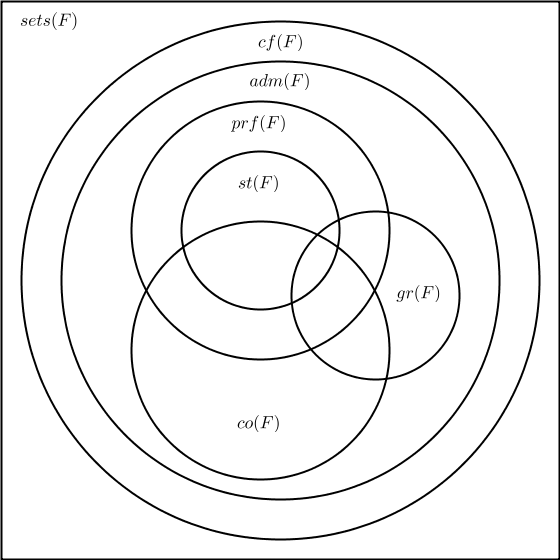
\includegraphics[scale=0.5]{pics/diagram.png}
		\caption{Relations between extensions}
	\end{figure}
\FloatBarrier

\chapter{Application}

\section{Introduction}
In this section the usage and implementation details of the aforementioned program illustrating the computation of the different extension types is provided. The application consists of two views: the input mask and the graph view.

\section{Input mask}
On starting the application the user is presented with an input mask. It consists of ten rows representing the arguments of an argumentation framework. The number of arguments is limited to ten because a higher number of arguments doesn't provide any further benefit to a user wanting to learn about the basics of argumentation frameworks.\\
Each row consists of a checkbox and two textfields.\hl
Each checkbox is labeled with the name of the argument the row represents. If a checkbox is selected the program will use the represented argument for further computations and visualisations.\hl
The first textfield of each row contains the optional description of the argument in question. The argument description is optional because it is only used in a cosmetic, non-functional way in the rest of the program.\hl
The second textfield of each row contains the names of the arguments the argument in question attacks. Argument names are case-insensitive and can be, but don't have to be, seperated either by ',' or spaces.\hl
The ``show graph'' button checks input in selected rows for problems. It detects attacks against non-existent arguments, while treating multiple attacks of an argument against another argument are ignored. It further provides error messages, so the user knows about issues. Note that unselected rows are ignored, even if there is a description or attacks already defined. This enables the user to quickly add or remove arguments for comparison in the next window.\hl
To make using the application easier, every item seen on screen shows a tooltip explaining the purpose of that element.

\FloatBarrier
	\begin{figure}[!htb]
		\centering
		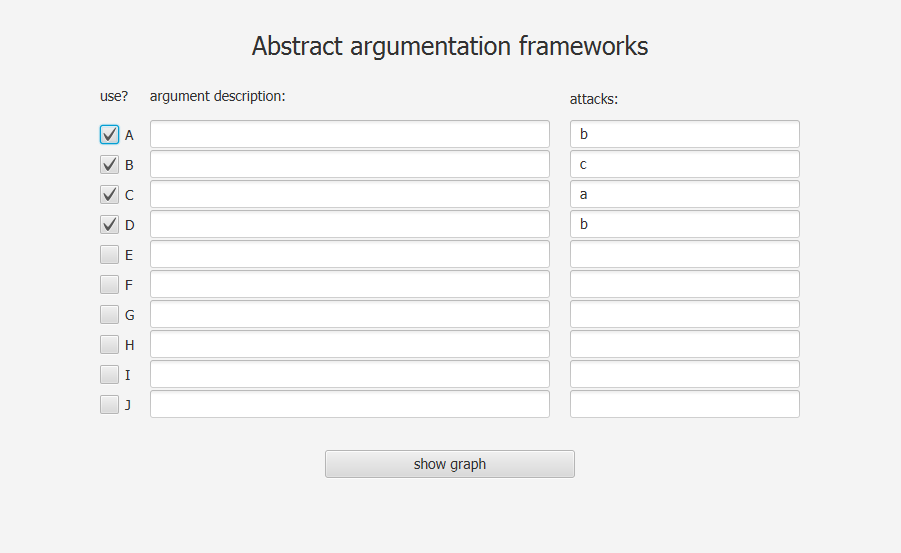
\includegraphics[width=\linewidth]{pics/input.png}
		\caption{Input mask}
	\end{figure}
\FloatBarrier

%TODO update figure name?
Figure 4.1 shows the input mask with input representing the argumentation framework $F=(A,R)$ with $A=\{a,b,c,d\}$ and $R=\{(a,b),(b,c),(c,a),(d,b)\}$.

\section{Graph view}
Once an argument framework is created, ``show graph'' clicked and no problems detected the graph view is shown.

\FloatBarrier
	\begin{figure}[!htb]
		\centering
		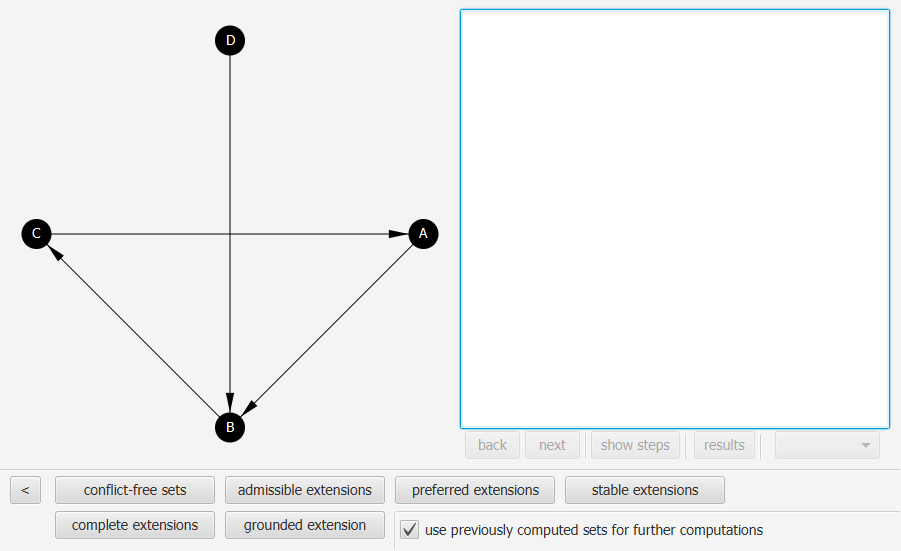
\includegraphics[width=\linewidth]{pics/demo.png}
		\caption{Graph view resulting from Figure 4.1}
	\end{figure}
\FloatBarrier

Upon loading the graph view the user can see the graph representing the argument framework defined in the input mask to the left. Every argument is represented by a node labelled with that arguments name. The argument nodes are laid out in a circle for better distinguishability.\hl
The user then has the option to choose to compute one of six extension types:

\begin{itemize}[noitemsep]
	\item conflict-free set
	\item admissible extension
	\item preferred extension
	\item stable extension
	\item complete extension
	\item grounded extension
\end{itemize}

If the checkbox to ``use previoucly computed sets for further computations'' is selected, each computation takes into account the results of preceding computations, if applicable. If this option is not selected the program will compute every extension type needed, prior to computing the chosen extension.\\
That means if conflict-free sets were already computed one can compute stable extensions without the need to compute conflict-free sets again, but when trying to compute preferred extensions the set of admissible extensions would have to be freshly computed (the computation of the admissible extensions using the already computed conflict-free extensions).\hl
Each computation triggers the text area (called the explanation area) to the right to display explanations of how the computed extensions came to pass. This explanation can either be shown step-by-step, all at once or be skipped and only the results be shown. Using previoucly computed extensions the explanation area does not show the explanation for already computed extensions again.

\FloatBarrier
	\begin{figure}[!htb]
		\centering
		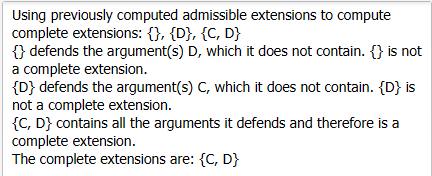
\includegraphics{pics/explanation.png}
		\caption{Text explaining the computation of admissible extensions.}
	\end{figure}
\FloatBarrier

To further illustrate the explanations shown the application recolors the graph for each step, using three easily distinguishable colors:\hl
Green is used for arguments included in the considered set and their relevant attacks needed to qualify for an extension type.\\
Red is used for conflicting arguments and attacks preventing a set of arguments from qualifying for an extension type.\\
Blue is used for arguments missing from a set for it to qualify for an extension type.\hl

\FloatBarrier
	\begin{figure}[!htb]
		\centering
		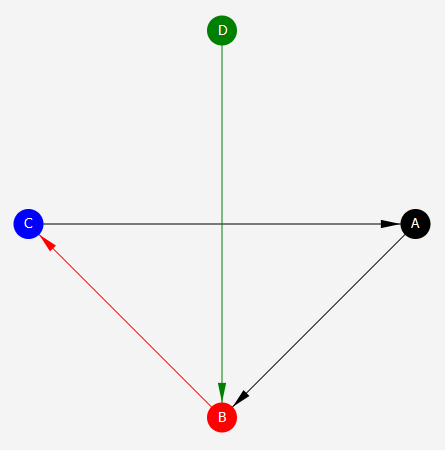
\includegraphics{pics/colored.png}
		\caption{\{A,D\} does not defend against C, so it is not an admissible extension.}
	\end{figure}
\FloatBarrier

After showing the results of a computation a dropdown menu becomes availiable to the right bottom side of the explanation area, containing all computed extensions. They can be selected and are then highlighted in green in the graph.\hl
The graph view also allows the user to go back to the input mask using the `<' button. The input mask will still contain the input from before switching to the graph view.

\subsection{Algorithms}
This section shows how the extension types are computed. For each type it is assumed that if a set of other extensions is prerequisite for the computation, this set already exists.

\subsubsection{Conflict-free sets}
text

\subsubsection{Admissible extensions}
text

\subsubsection{Stable extensions}
text

\subsubsection{Preferred extensions}
text

\subsubsection{Complete extensions}
text

\subsubsection{Grounded extension}
text

\backmatter

% Add a bibliography
\bibliographystyle{alpha}
\bibliography{intro}

% Add an index
\printindex

% Add a glossary
\printglossaries

\end{document}